\documentclass[12pt,a4paper]{article}
\usepackage[OT1]{fontenc}
\usepackage{amsmath}
\usepackage{amsfonts}
\usepackage{amssymb}
\usepackage{graphicx}
\usepackage{array}
\usepackage{cancel}
\usepackage{caption}
\usepackage{wrapfig}
\usepackage{secdot}
\usepackage{indentfirst}
\usepackage[left=1.5cm,right=1.5cm,top=0.3cm,bottom=1.5cm,includefoot,footskip=1.5cm]{geometry}
\usepackage[utf8]{inputenc}
\usepackage[english, russian]{babel}
\begin{document}
\textbf{
\begin{flushright}
Илья Кочергин, 626 группа
\end{flushright}}
\paragraph{\large Работа 3.3.6}
\paragraph{\Large Влияние магнитного поля на проводимость\\ полупроводников}
\paragraph{Цель работы:}измерение магнетосопротивления полупроводниковых образцов различной\\формы.
\paragraph{Оборудование:}стабилизированный источник постоянного тока и напряжения, электромагнит, цифровой вольтметр, амперметр, миллиамперметр, реостат, измеритель магнитной индукции Ш1-10, образцы (InSb) монокристаллического антимонида индия n-типа.
\section{Теоретическая справка}
\paragraph{Выражение для магнетосопротивления.} Рассмотрим проводник с током, помещенный в магнитное поле. Пусть его вектор индукции $\vec{B}$ направлен перпендикулярно вектору напряженности электрического поля $\vec{E}$ (эффектом Холла пренебрегаем). Тогда усредненное по времени уравнение движения в стационарном состоянии имеет вид (здесь и далее все скорости считаются \emph{усредненными по времени})
\begin{equation}
\vec{E} + \frac{\vec{v}}{b} + \vec{v}\times\vec{B} = 0\label{eq},
\end{equation}
здесь $b$~--- подвижность электронов, $\vec{v}$~--- скорость. Если электрическое поле направлено вдоль оси $x$, то отсюда получим выражение для проекции скорости электрона на эту ось:
\begin{equation}
v_x = -\frac{bE}{1+\left(bB\right)^2}
\end{equation}
Из этого выражения получаем эффективный коэффициент подвижности $b^*$:
\begin{equation}
b^* = -\frac{v_x}{E} = \frac{b}{1+\left(bB\right)^2}\label{eff}.
\end{equation}
Подставим это в формулу для удельного сопротивления $\rho$:
\begin{equation}
\rho = \frac{1}{enb^*} = \frac{1}{enb}\left(1+\left(bB\right)^2\right) = \rho_0\left(1+\left(bB\right)^2\right)\label{rho}, 
\end{equation}
где $\rho_0$ - удельное сопротивление в отсутствии магнитного поля. Таким образом, искомая зависимость квадратична, и линейна в координатах $\rho\left(B^2\right)$. Зависимость сопротивления $R$ от $B$ имеет такой же вид, т.к. $R = A\rho$, где $A$ зависит только от геометрических параметров.
\paragraph{Диск Корбино.} На самом деле, пренебрежение эффектом Холла при выводе формулы (\ref{rho}) неправильно, т.к. эффект Холла должен в точности компенсировать магнетосопротивление. Его наличие у проводников обуславливается тем, что Холловское напряжение компенсирует влияние только на электроны, движущиеся со скоростью, близкой к средней. Тем не менее, магнетосопротивление будет зависеть от ориентации. Поэтому в экспериментах обычно используют \emph{диск Корбино}. В нем напряженность внешнего электрического поля направлена радиально (контакты подсоединены к внешней и внутренней сторонам), а индукция магнитного поля~--- перпендикулярно плоскости диска. Магнитное поле вызывает дополнительное трансверсальное движение зарядов, которое не приводит к их накоплению. Отсюда $E_\text{х} = 0$ и формула (\ref{rho}) полностью применима. Если толщина диска $h$, а внешний и внутренний диаметры $D$ и $d$ соответственно, то сопротивление диска $R$ выражается по формуле
\begin{equation}
R_0 = \frac{\rho_0}{2\pi h}\ln\frac{D}{d}
\end{equation}
\section{Калибровка}
\begin{wrapfigure}{r}{0.52\textwidth}
\vspace{-40pt}
\centering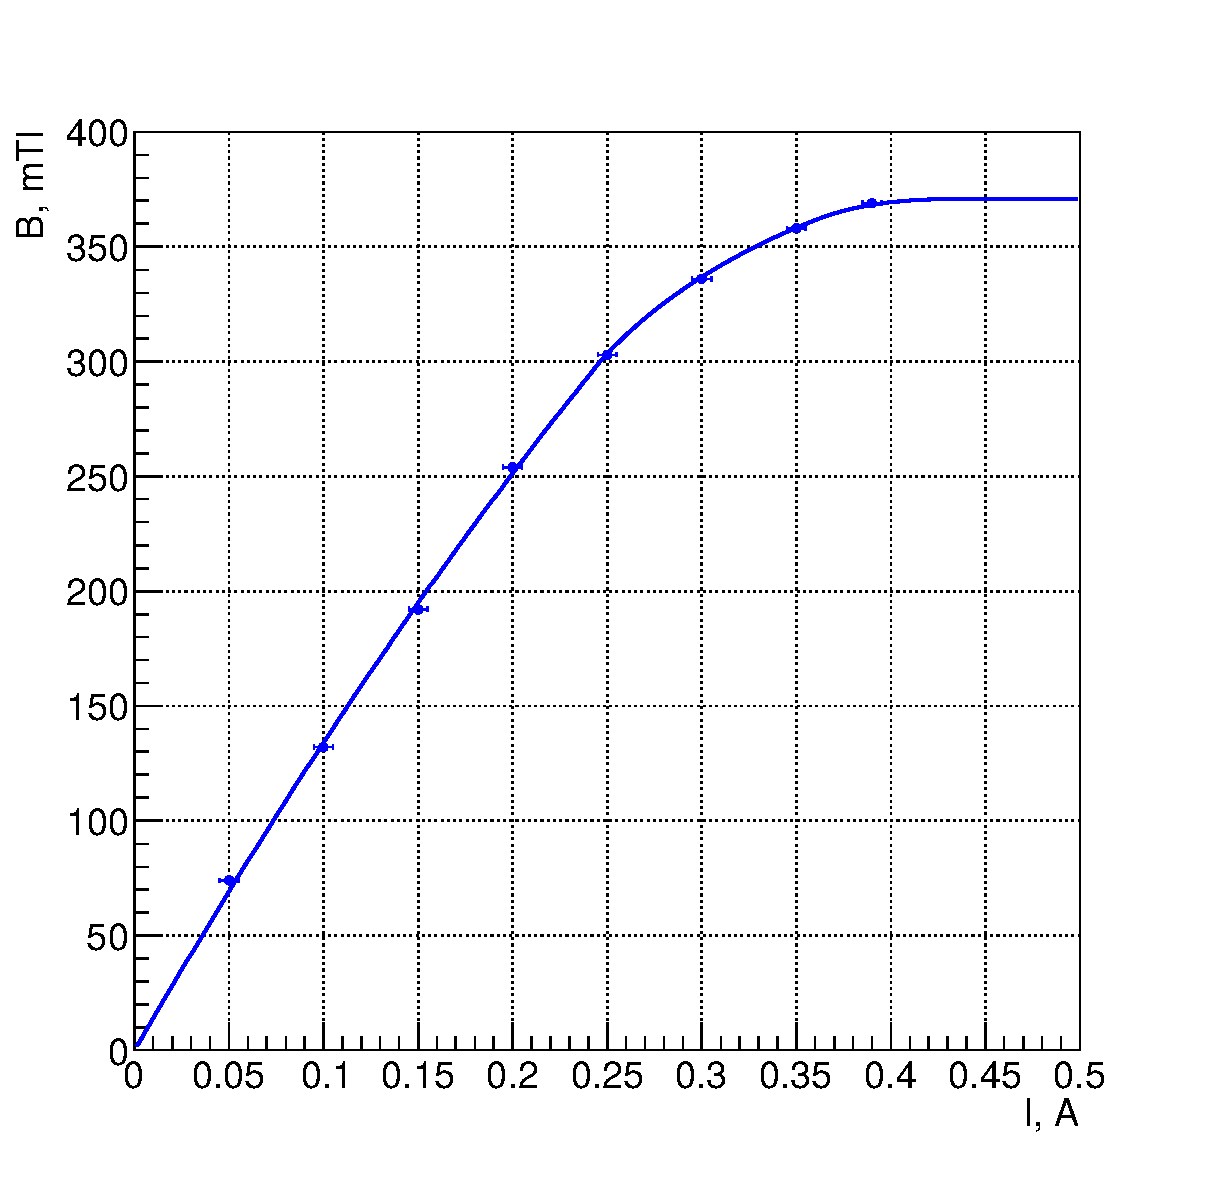
\includegraphics[width = 0.52\textwidth]{Plot1}
\captionsetup{justification = centering}
\caption{График зависимости $B(I)$\label{Fig1}}
\vspace{-15pt}
\end{wrapfigure}
\paragraph{Экспериментальная установка.} Установка в этой части практически полностью аналогично установке в соответствующей части работы 3.4.1 (вместо милливеберметра на данной установке используется датчик Холла, сразу измеряющий магнитное поле), поэтому не будем повторно приводить описание.
\paragraph{Обработка результатов} Результаты измерений $B(I)$ занесены в таблицу 1 (см. часть 3, ток обозначен $I_\text{м}$), график представлен на рисунке 1. Из него видно, что сердечник магнита почти достигает насыщения, поэтому придумать аппроксимирующую функцию довольно сложно (была проведена гладкая кривая).
\section{Исследование \\ магнетосопротивления}
\begin{wrapfigure}{r}{0.45\textwidth}
\centering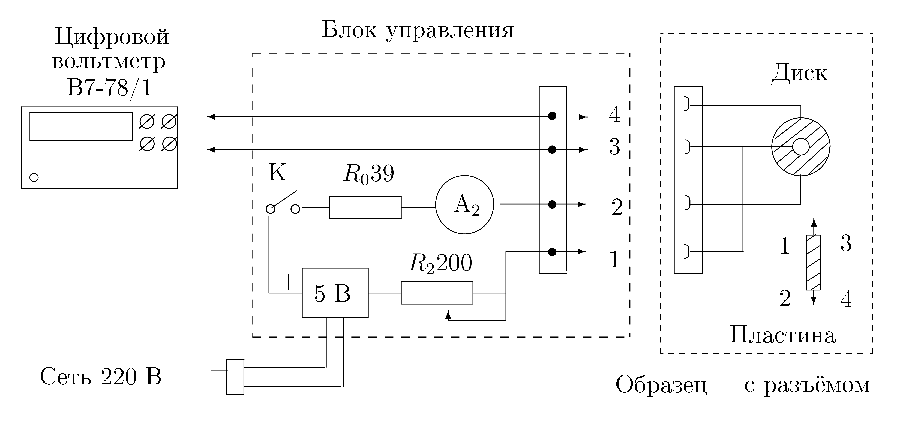
\includegraphics[width = 0.45\textwidth]{Pct1}
\captionsetup{justification = centering}
\caption{Схема установки \label{Fig2}}
\end{wrapfigure}
\paragraph{Экспериментальная установка.} Схема экспериментальной установки представлена на рис. 2. Ток $I$ через образец, измеряемый амперметром, регулируется реостатом $R_2$, т.к. его сопротивление достаточно большое, значение силы тока практически не меняется в ходе эксперимента. Вольтметр измеряет напряжение $U$ на образце. Таким образом, сопротивление измеряется формулой
\begin{equation}
R = \frac{U}{I},
\end{equation}
называемой \emph{законом Ома}. Согласно (4), зависимость $R\left(B^2\right)$ должна быть линейной. Для ее получения будем проводить измерения на тех же токах через электромагнит, при которых производилась калибровка.
\paragraph{Обработка результатов.} Экспериментальные данные вместе с пересчитанными результатами занесены в таблицу 1. Связь индексов с образцами следующая: 1~--- диск Корбино, 2~--- пластина с шириной вдоль магнитного поля, 3~--- пластина с шириной, перпендикулярной магнитному полю. Для диска $I = 25,0~\text{мА}$, для пластинки~--- $10,0~\text{мА}$. Погрешности (обозначены знаком $\Delta$) были вычислены по следующим формулам:
\begin{alignat}{1}
\Delta B &= 2~\text{мТл}; \\
\Delta U &= 0,02~\text{мВ}; \\
\Delta I &= 0,02~\text{мА}; \\ 
\Delta B^2 &= 2B^2\frac{\Delta B}{B}; \\
\Delta R &= R\sqrt{\left(\frac{\Delta I}{I}\right)^2 + \left(\frac{\Delta U}{U}\right)^2}.
\end{alignat}
\begin{table}[h!]\centering
\begin{tabular}{|*{10}{c|}}
\hline
$I_\text{м}, \text{мА}$&0&0,05&0,1&0,15&0,2&0,25&0,3&0,35&0,39\\
\hline
$B, \text{мТл}$&0&74&132&192&254&303&336&358&369\\
\hline
$B^2, \text{мТл}^2/10^3$&0&5,5&17,4&36,9&64,5&91,8&112,9&128,2&136,2\\
\hline
$\Delta B^2, \text{мТл}^2/10^3$&0&0,3&0,5&0,8&1,0&1,2&1,3&1,4&1,5\\
\hline
$U_1, \text{мВ}$&0,67&0,79&1,09&1,5&2,01&2,5&2,87&3,12&3,28\\
\hline
$U_2, \text{мВ}$&2,69&2,73&2,79&2,87&2,95&3,02&3,08&3,11&3,13\\
\hline
$U_3, \text{мВ}$&2,69&2,76&2,88&2,97&3,08&3,19&3,26&3,32&3,38\\
\hline
$R_1, \text{мОм}$&27&32&44&60&80&100&115&125&131\\
\hline
$\Delta R_1, \text{мОм}$&1&1&1&1&1&1&1&1&1\\
\hline
$R_2, \text{мОм}$&269&273&279&287&295&302&308&311&313\\
\hline
$\Delta R_2, \text{мОм}$&2&2&2&2&2&2&2&2&2\\
\hline
$R_3, \text{мОм}$&269&276&288&297&308&319&326&332&338\\
\hline
$\Delta R_3, \text{мОм}$&2&2&2&2&2&2&2&2&2\\
\hline
\end{tabular}
\caption{Все необходимые данные}
\end{table}
\begin{wrapfigure}{r}{0.52\textwidth}
\vspace{-20pt}
\centering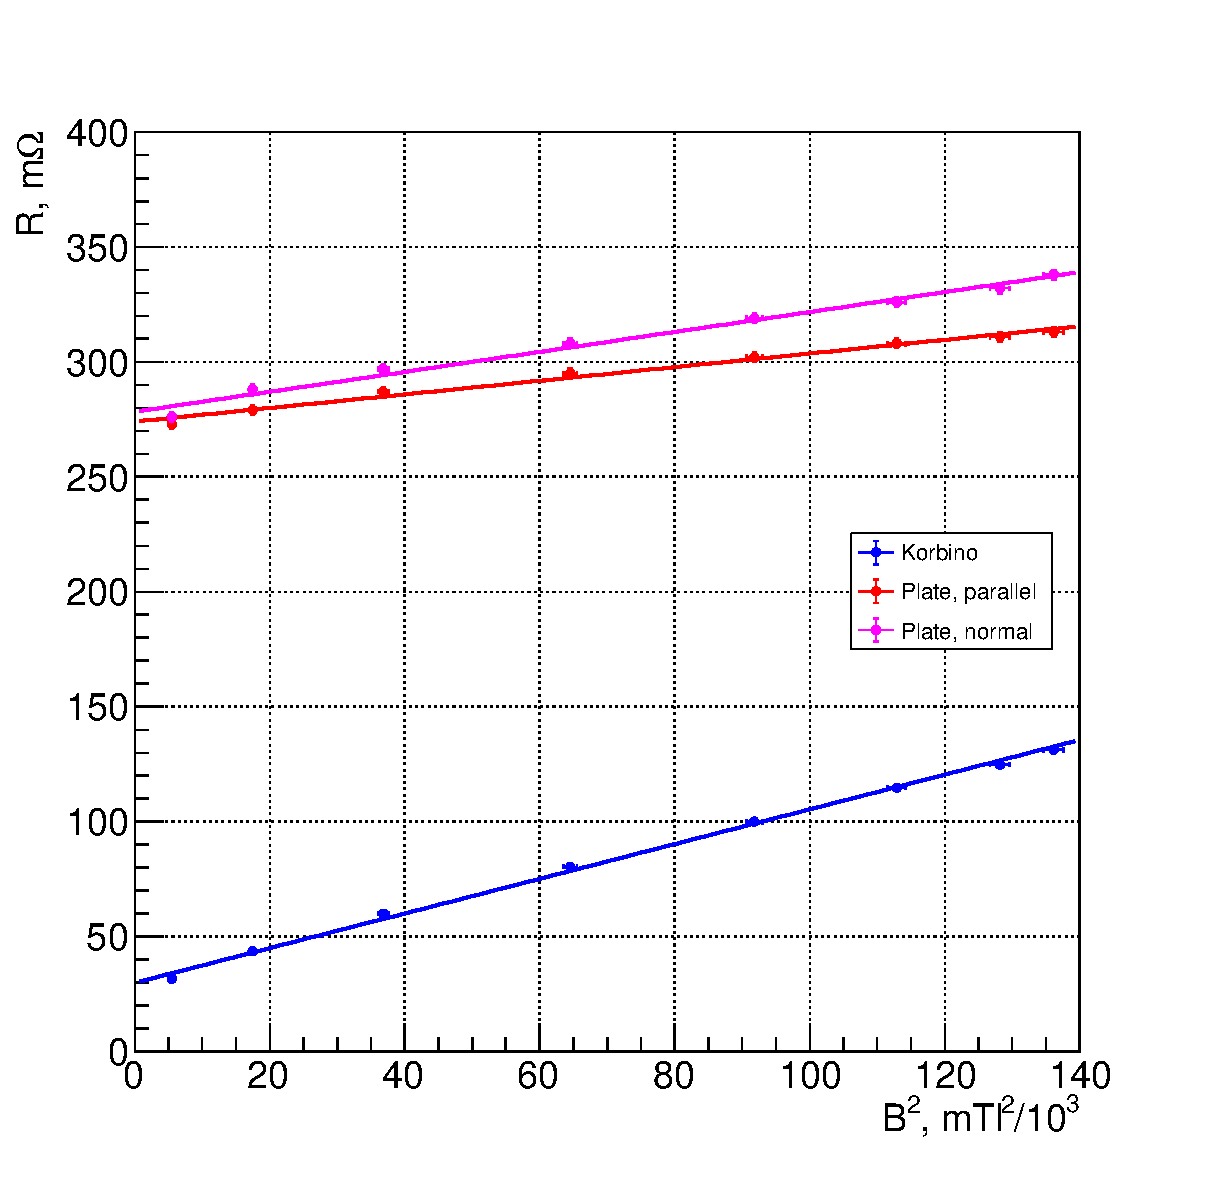
\includegraphics[width = 0.52\textwidth]{Plot2}
\captionsetup{justification = centering}
\caption{График зависимости $R(B^2)$\label{Fig3}}
\vspace{-20pt}
\end{wrapfigure}

\noindent Графики зависимостей $R\left(B\right)^2$ представлены на рис. 2. Это действительно прямые, причем для пластины нелинейные эффекты не проявляются. Из них находим подвижности, пользуясь (4):
\begin{equation}
b = \sqrt{\frac{k}{R_0}},
\end{equation}
где $k$~--- коэффициент наклона. Погрешности определяются выражением
\begin{equation}
\Delta b = \frac{b}{2}\sqrt{\left(\frac{\Delta k}{k}\right)^2 + \left(\frac{\Delta R_0}{R_0}\right)^2}.
\end{equation}
В итоге получим:
\begin{alignat}{1}
k &= (7,5 \pm 0,1)~\text{Ом} \text{Тл}^2; \\
b &= (5,3 \pm 0,3)~\text{1/Тл}.
\end{alignat}
Это значение близко к табличному (7,8~1/Тл). Теперь из (5) определим удельное сопротивление, предварительно записав параметры диска:
\begin{alignat}{1}
h &= 1,8~\text{мм};\\
d &= 3,0~\text{мм};\\
D &= 18,0~\text{мм};\\
\rho &= \frac{2\pi h R_0}{\ln \frac{D}{d}} = (1,7 \pm 0,1)\cdot 10^{-4}~\text{Ом}\cdot\text{м}\\
\Delta \rho &= \frac{\Delta R_0}{R_0} \rho.
\end{alignat}
\section{Вывод}
Цели работы были достигнуты, все величины были определены, хотя они и не очень хорошо сходятся с табличными.
\end{document}

